% Fuente: Pauta del Auxiliar 10, «KKT — Pregunta 1».
Lo primero que corresponde hacer antes de utilizar las condiciones de KKT es verificar que se cumplan las hipótesis que aseguran la \textbf{suficiencia}:

\begin{itemize}
  \item \textbf{Funciones diferenciables:} Tanto la función objetivo (\(J\)) como las funciones que definen las restricciones de igualdad y desigualdad (\(h\) y \(f\)) son diferenciables.

  \item \textbf{Problema convexo:} El problema es convexo pues la función \(J\) es convexa (forma cuadrática con matriz definida positiva)\footnote{También se puede concluir esto si se tiene en cuenta que la operación suma mantiene la convexidad de las funciones y las funciones sumadas son todas convexas.}, la restricción de desigualdad es convexa (es una función afín) y la restricción de igualdad es afín.

  \item \textbf{Condición de Slater:} Se cumple, basta con elegir un punto \(\hat{x}\) que cumpla con \(f(\hat{x}) = \hat{x}_4 - A < 0\) y que satisfaga la restricción de igualdad. El punto \(\hat{x}(x_4) = (-x_4+1,\, 0,\, 0,\, x_4)\) siempre satisface la restricción de igualdad y eligiendo \(x_4 = A - \varepsilon\) se garantiza que \(f(\hat{x}) < 0\).

  \item \textbf{Dualidad fuerte:} Como se tiene la condición de Slater y el problema es convexo se asegura la dualidad fuerte.
\end{itemize}

Estas hipótesis son suficientes para que una solución que cumpla con las condiciones de KKT sea óptima para el primal y dual. De esta forma, teniendo en cuenta el lagrangiano del problema,
\[
L = x_1^2 + x_2^2 + x_3^2 + x_4^2 + \mu (1 - x_1 - x_2 - x_3 - x_4) + \lambda (x_4 - A)
\]

Se obtienen las siguientes condiciones de KKT:

\begin{align*}
  \left( \frac{\partial L}{\partial x_1} = 0\right) \Rightarrow &\:2x_1 - \mu = 0 \\
  \left( \frac{\partial L}{\partial x_2} = 0 \right)\Rightarrow &\:2x_2 - \mu = 0 \\
  \left( \frac{\partial L}{\partial x_3} = 0 \right) \Rightarrow &\: 2x_3 - \mu = 0 \\
  \left( \frac{\partial L}{\partial x_4} = 0 \right) \Rightarrow &\: 2x_4 - \mu + \lambda = 0 \\
  &x_1 + x_2 + x_3 + x_4 = 1 \\
  &x_4 \leq A \\
  &\lambda \geq 0 \\
  &\lambda (x_4 - A) = 0
\end{align*}

A partir de las ecuaciones de optimalidad es posible deducir que,
\[
x_1 = x_2 = x_3 = \frac{\mu}{2}, \qquad x_4 = \frac{\mu - \lambda}{2}
\]

Con esto y con la restricción de igualdad es posible despejar \(\mu\) para dejar todo en función de \(\lambda\) \emph{(esto hace que sea más simple verificar la positividad de la variable dual)}:
\[
x_1 + x_2 + x_3 + x_4 = 4\left( \frac{\mu}{2} \right) - \frac{\lambda}{2} = 1
\quad \Rightarrow \quad
\mu = \frac{2 + \lambda}{4}
\]

Reemplazando \(\mu\) en las variables primales del problema se obtiene,

\begin{equation}
   x_1 = x_2 = x_3 = \frac{2 + \lambda}{8},
\qquad
x_4 = \frac{2 + \lambda}{8} - \frac{\lambda}{2} = \frac{1}{4}-\frac{3\lambda}{8}
\label{ex:6:4:eq1} 
\end{equation}

Como ya hemos dejado los valores de las variables primales en función de \(\lambda\) (que es una variable dual positiva), utilizamos la inecuación del problema primal (condiciones de factibilidad del primal),
\begin{equation}
    x_4 \leq A
\Rightarrow
\frac{1}{4}-\frac{3\lambda}{8} \leq A
\Rightarrow
\frac{1}{4}-A \leq \frac{3\lambda}{8}
\label{ex:6:4:eq2}
\end{equation}


Dado que queremos resolver el problema para todos los valores de \(A\), lo razonable es estudiar los resultados que se obtienen para diferentes rangos de valores de \(A\). A partir del resultado de \ref{ex:6:4:eq2} podemos darnos cuenta que hay dos casos que vale la pena estudiar: cuando \(A \geq \frac{1}{4}\), pues la restricción \(x_4 \leq A\) se vuelve redundante; y cuando \(A < \frac{1}{4}\), pues la restricción \(0 \leq \lambda\) se vuelve redundante. Es decir,
\[
\left\{
\begin{array}{ll}
\frac{1}{4} - A \leq 0 \leq \frac{3\lambda}{8} & \text{Si } A \geq \frac{1}{4} \\
0 < \frac{1}{4} - A \leq \frac{3\lambda}{8} & \text{Si } A < \frac{1}{4}
\end{array}
\right.
\]

\noindent
\textbf{Caso \(A \geq \frac{1}{4}\):} La restricción \(x_4 \leq A\) (ecuación \ref{ex:6:4:eq2}) se satisface siempre si la restricción \(0 \leq \lambda\) se cumple. Por esta razón, condicionamos sobre los valores que puede tomar \(\lambda\):

\begin{itemize}
  \item \(\lambda > 0\): Para satisfacer la restricción de holgura complementaria \((\lambda(x_4 - A) = 0)\) se requiere que la restricción \ref{ex:6:4:eq2} se cumpla con igualdad, sin embargo, se llega a una contradicción,
  \[
    \frac{1}{4}-A = \frac{3\lambda}{8} \quad \text{pero} \quad \frac{1}{4}-A \leq 0 \Rightarrow \lambda \leq 0 \wedge \lambda > 0
  \]
  \emph{Debido a que se llega a una contradicción, no es posible encontrar una solución si \(\lambda > 0\).}
    
  \item \(\lambda = 0\): Se garantiza la condición de holgura complementaria y al calcular la solución del problema primal \ref{ex:6:4:eq1} se obtiene,
  \[
    x_1 = x_2 = x_3 = x_4 = \frac{1}{4}
  \]
\end{itemize}

Con lo anterior, nos damos cuenta que,
\[
J(x^*) = \frac{1}{4}
\]

\noindent
\textbf{Caso \(A < \frac{1}{4}\):} En este caso siempre se tiene que \(\lambda > 0\) pues,
\[
0 < \frac{1}{4} - A \leq \frac{3\lambda}{8}
\]

Por esta razón, para cumplir con la condición de holgura complementaria, se requiere que \(x_4 = A\). Utilizando la restricción de igualdad se obtiene,
\[
x_1 = x_2 = x_3 = \frac{1 - A}{3}
\]

Así, se tiene que,
\begin{align*}
J(x^*) &= 3\left( \frac{1}{9}(1 - A)^2 \right) + A^2 \\
&= \frac{1}{3}\left( 4A^2 - 2A + 1 \right)
\end{align*}

A partir del análisis anterior, el costo óptimo del problema de optimización corresponde a:
\[
\min J = 
\begin{cases}
\frac{1}{4} & \text{Si } A \geq \frac{1}{4} \\
\frac{1}{3}(4A^2 - 2A + 1) & \text{Si no}
\end{cases}
\]

Se observa que cuando \(A \geq \frac{1}{4}\), la restricción de desigualdad se vuelve irrelevante, pues nunca se activa. Esto se puede constatar en la resolución del problema dado que la restricción \(\lambda \geq 0\) es más exigente que \(x_4 \leq A\) si \(A \geq \frac{1}{4}\).

\begin{figure}
    \centering
    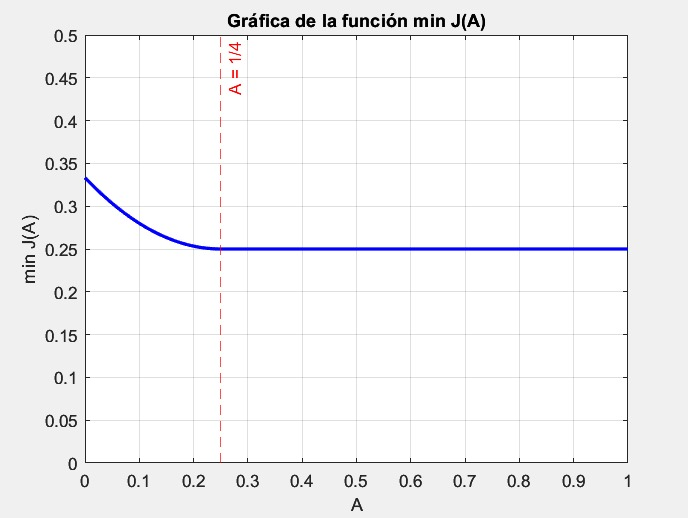
\includegraphics[width=0.5\linewidth]{img/ejercicios/Capitulo-6/ejercicio_6_4_min_j.jpeg}
    \caption{Gráfica función min J(A)}
    \label{ex:6:4:fig:min-j}
\end{figure}
